\documentclass[fleqn]{article}

\usepackage{amsmath}
\usepackage{amsfonts}
\usepackage[utf8]{inputenc}
\usepackage[top=2.5cm, bottom=4cm, left=2cm, right=2cm]{geometry}
\usepackage[francais]{babel}
\usepackage{perpage}
\usepackage[toc,page]{appendix} 
\MakePerPage{footnote}
\usepackage{color}
\usepackage{algorithmic}
\usepackage{amsmath}
\usepackage{amsfonts}
\usepackage{fancyhdr}
\usepackage{enumitem}
\usepackage{parskip}

\usepackage{multicol}
\usepackage{graphicx}

\pagestyle{fancy}
\renewcommand{\headrulewidth}{1pt}
\fancyhead[L]{Algèbre Linéaire Numérique}
\fancyhead[C]{}
\fancyhead[R]{Nguyen - Boukraichi - Démery}
\renewcommand{\footrulewidth}{1pt}
\fancyfoot[L]{ENSEEIHT IMA 1N}
\fancyfoot[C]{- \thepage -}
\fancyfoot[R]{19 Mai 2017}
\setlength{\parskip}{8pt}


\newenvironment{itemize*}%
  {\begin{itemize}[label=\textbullet]%
    \setlength{\itemsep}{5pt}%
    \setlength{\parskip}{5pt}}%
  {\end{itemize}}
  
  \newenvironment{enum}%
  {\begin{enumerate}%
    \setlength{\itemsep}{10pt}%
    \setlength{\parskip}{5pt}}%
  {\end{enumerate}}
 

\title{\textit {Projet d'Informatique et Mathématiques Appliquées \\
Algèbre Linéaire Numérique}}
\date{}
\author{BOUKRAICHI Hamza,
DEMERY Cyril,
NGUYEN Teo}

\begin{document}

\maketitle

\section{Deliverables phase 2}

\subsection{Introduction}

Dans ce problème, nous avons voulu prévoir l'évolution dans le temps et l'espace de l'atmosphère à travers un modèle simplifié.

Le système d'équations non linéaires de Navier-Stokes ne possédant pas de solution analytique, nous sommes obligés d'approcher la solution. Pour calculer cette solution approchée, on construit une base de l'espace de la solution puis on construit une solution approchée à partir des données qu'on possède.

Comme le problème de l'atmosphère est de grande dimension, on construit plutôt un sous-espace dans lequel on va approcher la solution.
Cette approximation fait intervenir le calcul des vecteurs singuliers et nécessite ainsi le calcul de la SVD. Cependant, le calcul de la SVD est très couteux et n'est pas efficace dans un problème de grande dimension.

Dans ce projet, nous cherchons à trouver une implémentation efficace afin de calculer les valeurs singulières (et leurs vecteurs propres associés) d'une matrice, afin de trouver une solution approchée du problème en un temps convenable. Ce calcul se fait en utilisant la projection de Rayleigh-Ritz et avec un algorithme adapté de celui de la puissance itérée. Alors que dans le dernier algorithme, on calcule les éléments propre un à un, avec notre algorithme adapté, nous sommes en capacité de calculer plusieurs éléments propres par itération.

Comme les calculs de cet algorithme se font sur une matrice $A \in \mathcal M _{n\times n}$ qui doit être symétrique, et que nous possédons simplement une matrice $Z \in \mathcal M _{m \times n}$, nous appliquons notre algorithme sur la matrice $Z^TZ$ (qui est symétrique). Or, le calcul de notre algorithme adapté de la puissance itérée se fait en multipliant par la matrice $A$ plusieurs fois (c'est à dire en multipliant par $A^p , p\geq 2$ : technique de l'itération par bloc). Nous devons donc calculer le produit $(Z^TZ)^p$; celui-ci pouvant être calculé de plusieurs manières différentes, nous avons cherché quelle était la manière la plus optimale de faire ce calcul.

\pagebreak

\subsection{Description de l'algorithme de calcul des éléments singuliers}

Dans l'algorithme implanté, on effectue $Y = Z^TZZ^TZ\cdots Z^T V$ (ou $Y=ZZ^TZ\cdots Z^TZV$ en fonction de la dimension de $V$), par similarité avec l'algorithme de la puissance itérée qui effectue une simple opération : $Y = AV$. On multiplie par $p$ matrices afin de pouvoir calculer plusieurs éléments singuliers à la fois.

Il faut par ailleurs normaliser les colonnes de $Y$ pour éviter que la convergence se fasse vers le vecteur singulier dominant. Ainsi, on normalisant, les colonnes de $Y$ convergeront équitablement vers des directions différentes. 

La version implantée possède une optimisation par rapport à la simple version où l'on ne cherche les vecteurs singuliers que d'un côté. En effet, notre algorithme "alterne" la recherche entre le vecteur singulier droite et gauche, afin de faire converger les deux. On est donc assuré de l'optimalité de l'algorithme puisqu'il va converger à la vitesse à laquelle le plus rapide des deux côtés convergerait.
Comme on ne sait pas en avance lequel des deux converge le plus vite, on fait la convergence alternée des deux.

$currentS$ permet de gérer la dimension de $V$, permettant de savoir si on doit effectuer le produit en terminant par $Z$ ou par $Z^T$.

Passer par le quotient de Rayleigh $H = V^TAV$ permet de trouver un sous-espace propre de $A$. Puis on effectue simplement la décomposition spectrale de $H$ ($H = X\Lambda X^T$), afin de trouver un sous-espace propre $X$ de $H$. En effet, la décomposition spectrale de $H$ est plus facile à obtenir que celle de $A$ car $H$ est de dimension $l \times l$ alors que celle de $A$ est $m \times m$ (ou $n \times n$), et $l < n < m$.  
\`A partir de ce dernier, on accède au sous-espace propre de $A$ en effectuant $V*X$.

On va ensuite tester la précision de la valeur propre approximée en exprimant 
$\displaystyle \frac{||Av_i - \lambda_iv_i||}{||A||}$.
On ne considère que les valeurs propres avec une précision suffisante (une erreur relative petite).

Enfin, on continue la boucle jusqu'à ce qu'on ait dépassé le nombre maximal d'itérations qu'on s'était fixé ($MaxIter$) ou que l'on ait trouvé un nombre suffisant de valeur propre ($PercentReached$). Ce pourcentage est obtenu en effectuant le rapport de la valeur propre actuellement considérée ($\lambda_i$) sur la valeur propre la plus grande. En effet, les valeurs propres étant rangées par ordre décroissant, $\lambda_1$ sera la plus grande valeur propre ; plus on avance dans l'algorithme, plus on trouve des valeurs propres petites (si $i$ augmente, $\lambda_i$ diminue). 

Ainsi, la somme $\displaystyle 1 - \sqrt \frac{\lambda_i}{\lambda_1}$ va tendre vers 1, assurant que l'on dépasse à un moment le pourcentage cherché ($percentInfo$).

\'Etant donné que l'on garde un compteur du nombre de valeurs propres qui ont convergé, on peut afficher à la fin toutes les valeurs singulières cherchées (la racine de toutes les valeurs propres trouvées).
Par ailleurs, grâce aux valeurs singulières on peut ensuite calculer les vecteurs singuliers gauche et droite.

~\\

Afin d'optimiser la complexité spatiale, on préfère réutiliser des matrices dont l'espace a déjà été aloué, plutôt que d'alouer un autre espace puis de le libérer. 

Ainsi, lors du calcul de $Z*Z'$ (ou $Z'*Z$ selon la valeur de $currentS$), on utilise l'espace déjà aloué par $U_{out}$ ; on n'en a en effet pas besoin puisqu'on le calcule à la fin grâce à la valeur de $V$.

De même, pour la décomposition spectrale de $H$, on utilise $Z$ comme espace de stockage, étant donné qu'on n'en a plus besoin (on a déjà calculé $Z^TZ$, ou $ZZ^T$). 

On utilise de nouveau $Z$ comme espace de stockage afin de de trier les valeurs propres par ordre décroissant (au lieu de l'ordre croissant initialement donné). 

Lors du calcul de la norme de $Av_i - \lambda_iv_i$, on utilise une fois de plus l'espace de $Z$.

Par ailleurs, lors de notre implémentation, nous avons choisi de calculer la trace de $Z^TZ$ au lieu de celle de $Z^TZ$ pour avoir une matrice moins grande à stocker ($50\times50$ au lieu de environ $ 270 000 \times 270 000$) et ainsi réduire la compléxité spatiale.




\pagebreak
\subsection{Tests de performance}

Les tests effectués sont les suivants : 

\begin{enumerate}
  \item Pour $p$ égaux, la performance de notre algorithme est moins bonne que celle des autres.
    \begin{itemize} 
      \item Pour $p=2, m=1000$, $n=500$, $l=200$, la version "sv\_both" donne 71 valeurs singulières (96\%) en 0.42 secondes, alors que notre version donne 13 valeurs singulières (24.2\%) en 1.24 secondes
      \item Pour $p=2, m=2000$, $n=1000$, $l=500$, la version "sv\_both" donne 288 valeurs singulières (99.9\%) en 4.98 secondes, alors que notre version donne 196 valeurs singulières (89.4\%) en 13.77 seconds.
      \item Pour $p=4, m=1000, n=500, l=200$, la version "sv\_left" donne 153 valeurs singulières (99\%) en 0.98 secondes, alors que notre version donne 32 valeurs singulières (43\%) en 0.85 secondes.
    \end{itemize}
\end{enumerate}

Plus globalement, on peut distinguer les cas entre $p$ petit et un $p$ plus grand. Par exemple, les diagrammes suivant montrent bien cette différence :

\begin{figure}[h]
\centering
\includegraphics[scale = 0.5]{p2vs.jpg}
\caption{Nombre de valeurs singulières trouvées en fonction de $m$ pour $p=2$}
\end{figure}

\begin{figure}[h]
\centering
\includegraphics[scale = 0.5]{p2temps.jpg}
\caption{Temps de convergence en fonction de $m$ pour $p=2$}
\end{figure}

\pagebreak

\begin{figure}[h]
\centering
\includegraphics[scale = 0.5]{p6vs.jpg}
\caption{Nombre de valeurs singulières trouvées en fonction de $m$ pour $p=6$}
\end{figure}

\begin{figure}[h]
\centering
\includegraphics[scale = 0.5]{p6temps.jpg}
\caption{Temps de convergence en fonction de $m$ pour $p=6$}
\end{figure}

Pour $p=6$, les versions 3 et 4 ne convergent pas, alors que notre version de l'algorithme converge (même si le nombre de valeurs singulières trouvées est faible). 

Le nombre de valeurs singulières trouvées en général par notre version est faible mais son temps de convergence reste très faible et il converge bien plus souvent que les versions 3 et 4.






\pagebreak
\subsection{\'Evaluation de l'algorithme avec la fonction Matlab de reconstruction}

En utilisant la fonction de reconstruction Matlab fournie, on peut comparer nos résultats avec les résultats obtenus avec l'utilisation de la fonction Matlab $svd$.

\begin{figure}[h]
\centering
\includegraphics[scale = 0.4]{matlab_resultat.jpg}
\caption{Résultats obtenus pour la reconstruction}
\end{figure}

On obtient 7 valeurs singulières en 8 secondes, avec une erreur de 2%.

\begin{figure}[h]
\centering
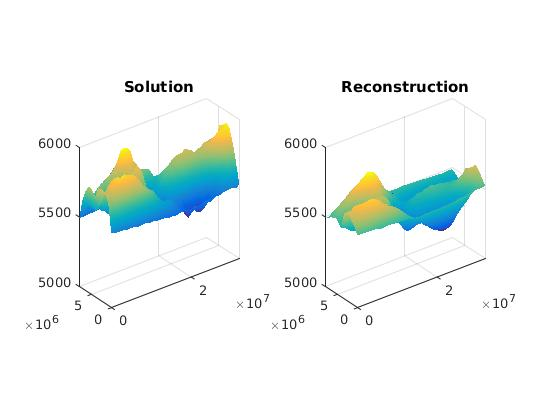
\includegraphics[scale = 0.4]{matlab_svd.jpg}
\caption{Résultats théoriques avec la fonction SVD}
\end{figure}

On obtient 4 valeurs singulières en 0.9 secondes, avec une erreur de 2%.

L'algorithme 1 permet d'améliorer la vitesse et la précision de la reconstruction de la manière suivante :

Vu la différence de vitesse de convergence entre le calcul des vecteurs singuliers gauches et droites, et vu que cette information n'est pas accessible (les vecteurs qui convergent en moins d'itérations), 
alterner entre le calcul des vecteurs droits et gauches permet de tester la convergence de chacun à chaque itération et de s'arrêter  grâce aux premiers vecteurs convergents. La mise a jour des matrices $U$ et $V$ à chaque itérations grâce à la relation :

$$ Zv = \sigma_1u $$ 
$$ Z^Tu = \sigma_1v $$

permet de transmettre les informations calculées à l'itérations précédentes et de maintenir cette relation vraie, ce qui en conséquent permet d'accroître la précision de l'algorithme. Alors que la fonction matlab SVD calcule tous les valeurs, vecteurs singuliers droits et gauches sans soucis de convergence, ce qui implique des calculs supplémentaires et inutiles qui deviennent pénalisants temporellement lorsque la taille des matrices augmente.

\pagebreak

\subsection{Conclusion}

Ce projet nous a permi de voir d'autres méthodes de résolution de systèmes différentiels qui ne possèdent pas de solution analytique. Nous avons pu apréhender les problèmes de grandes dimensions, représentatifs des problèmes typiques de mécanique des fluides, tout en appliquant les théorèmes vus en cours d'Algèbre Linéaire Numérique et d'Optimisation, ce qui nous a aussi permi de comprendre l'utilité de réduire la compléxité numérique et spatiale d'un algorithme de calcul. 


\end{document}
